\documentclass[aspectratio=169]{beamer}

% Default packages
\usepackage[T1]{fontenc}
\usepackage[utf8]{inputenc}
\usepackage[english]{babel}
\usepackage{pgfplots}
\pgfplotsset{compat=newest}
\usepackage{booktabs}
\usepackage{siunitx}
\usepackage{amsmath}
\usepackage{graphicx}
\usepackage{tikz}
\DeclareMathOperator*{\argmax}{arg\,max}
\DeclareMathOperator*{\argmin}{arg\,min}
\usepackage{dsfont}
\newcommand{\brilliantBlue}{blue!60!black}
\usepackage{colortbl}
\def \threeFoldCV{

    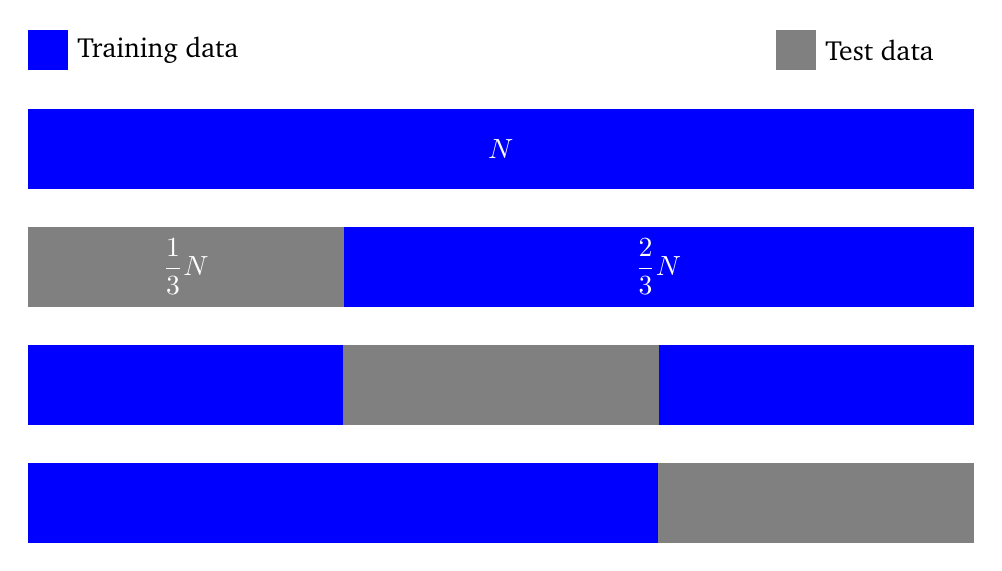
\begin{tikzpicture}
    
        %First line
        \filldraw[draw=blue, fill=blue] (0,3.5) rectangle (12,4.5);
        % third line
        \filldraw[draw=blue, fill=blue] (0,2) rectangle (12,3);
        \filldraw[draw=gray, fill=gray] (0,2) rectangle (4,3);
        %fourth line
        \filldraw[draw=blue, fill=blue] (0,0.5) rectangle (12,1.5);
        \filldraw[draw=gray, fill=gray] (4,0.5) rectangle (8,1.5);
        %fith line
        \filldraw[draw=blue, fill=blue] (0,-1) rectangle (12,0);
        \filldraw[draw=gray, fill=gray] (8,-1) rectangle (12,0);
        %Legend
        \node[] at (6,4) {\textcolor{white}{$N$}};
        
        \node[] at (2,2.5) {\textcolor{white}{$\dfrac{1}{3}N$} };
        \node[] at (8,2.5) {\textcolor{white}{$\dfrac{2}{3}N$} };
        
        \filldraw[draw=blue, fill=blue] (0,5) rectangle (0.5,5.5);
        \node[anchor=west] at (0.5,5.25) {Training data};
        
        \filldraw[draw=gray, fill=gray] (9.5,5) rectangle (10,5.5);
        \node[anchor=west] at (10,5.25) {Test data};
        
        
    \end{tikzpicture}

}

% Font selection
% Latin Modern
\usepackage{lmodern}
% Verdana font type
%\usepackage{verdana}
% Helvetica
%\usepackage{helvet}
% Times (text and math)
%\usepackage{newtx, newtxmath}
% Nice font combination
%\usepackage{mathptmx} % math
%\usepackage{sourcesanspro} % sans-serif
\usepackage{charter} % serif

% Use DTU theme, see below for options
\usetheme[department=compute]{DTU}

\title[DTU Templates]{Customer Identification in a Jiffy with Celebrus}
\author{Victor Elkjær Birk \& William Frisch Møller}
\institute{DTU Compute, Technical University of Denmark (DTU)}
\date{\today}
	
\newcommand{\tabitem}{{\color{dtured}$\bullet$} }

\begin{document}
\frame{
	\maketitle
}

\frame{
	\frametitle{Outline}
	\tableofcontents
}

\section{Motivation}
\frame{
	\frametitle{Time is money}
	\setbeamercovered{transparent}
	\onslide<1->{\begin{block}{Question}
	    \textit{To what extent can we improve our ability to tell customer from non-customer behavior as we
        collect more data through time?}
	\end{block}
	}
	\onslide<2->{\begin{block}{Why?}
	    Quickly identifying customers from non-customers opens up the possibility for targeted advertising.
	\end{block}
	}
    \onslide<3->{\begin{block}{Hypothesis}
	    As we gather more data, we should be able to get a better and better indication of whether the user in question is a customer or not.
	\end{block}
	} 
    \onslide<4->{\begin{block}{How did we test our hypothesis?}
        We created four datasets. These were constructed by aggregating data over time for each \texttt{sessionnumber}. We considered the following times: 0s, 5s, 60s and 300s and evaluated how the performance increased with the amount of data collected.
	\end{block}
	}
}

% Exec summary.  
% \frame{
%     \frametitle{Executive Summary}
%     \begin{itemize}
%         \item Ou
%     \end{itemize}
% }

\section{Data Handling}
\frame{
	\frametitle{A tedious journey from SQL to Excel and back}
    \begin{figure}
        \centering
        \includegraphics[width=0.8\linewidth]{fig/Data_prep.png}
    \end{figure}
    
    }
    \frame{
    \frametitle{A tedious journey from SQL to Excel and back}
    \begin{block}{Aftermath}
        After the data sets are created in SQL, they are imported in Python through the use of the \texttt{pandas} library, after which the final data adjustments are made. These include one-hot encoding and F-tests which transform categorical features to numerical, and removes the least significant ones, respectively, leaving us with 100 final features. 
    \end{block}
    }

\frame{
    \frametitle{Data examination I}
        \begin{columns}[T] % align columns
        \begin{column}{.33\textwidth}
        \begin{figure}
            \centering
            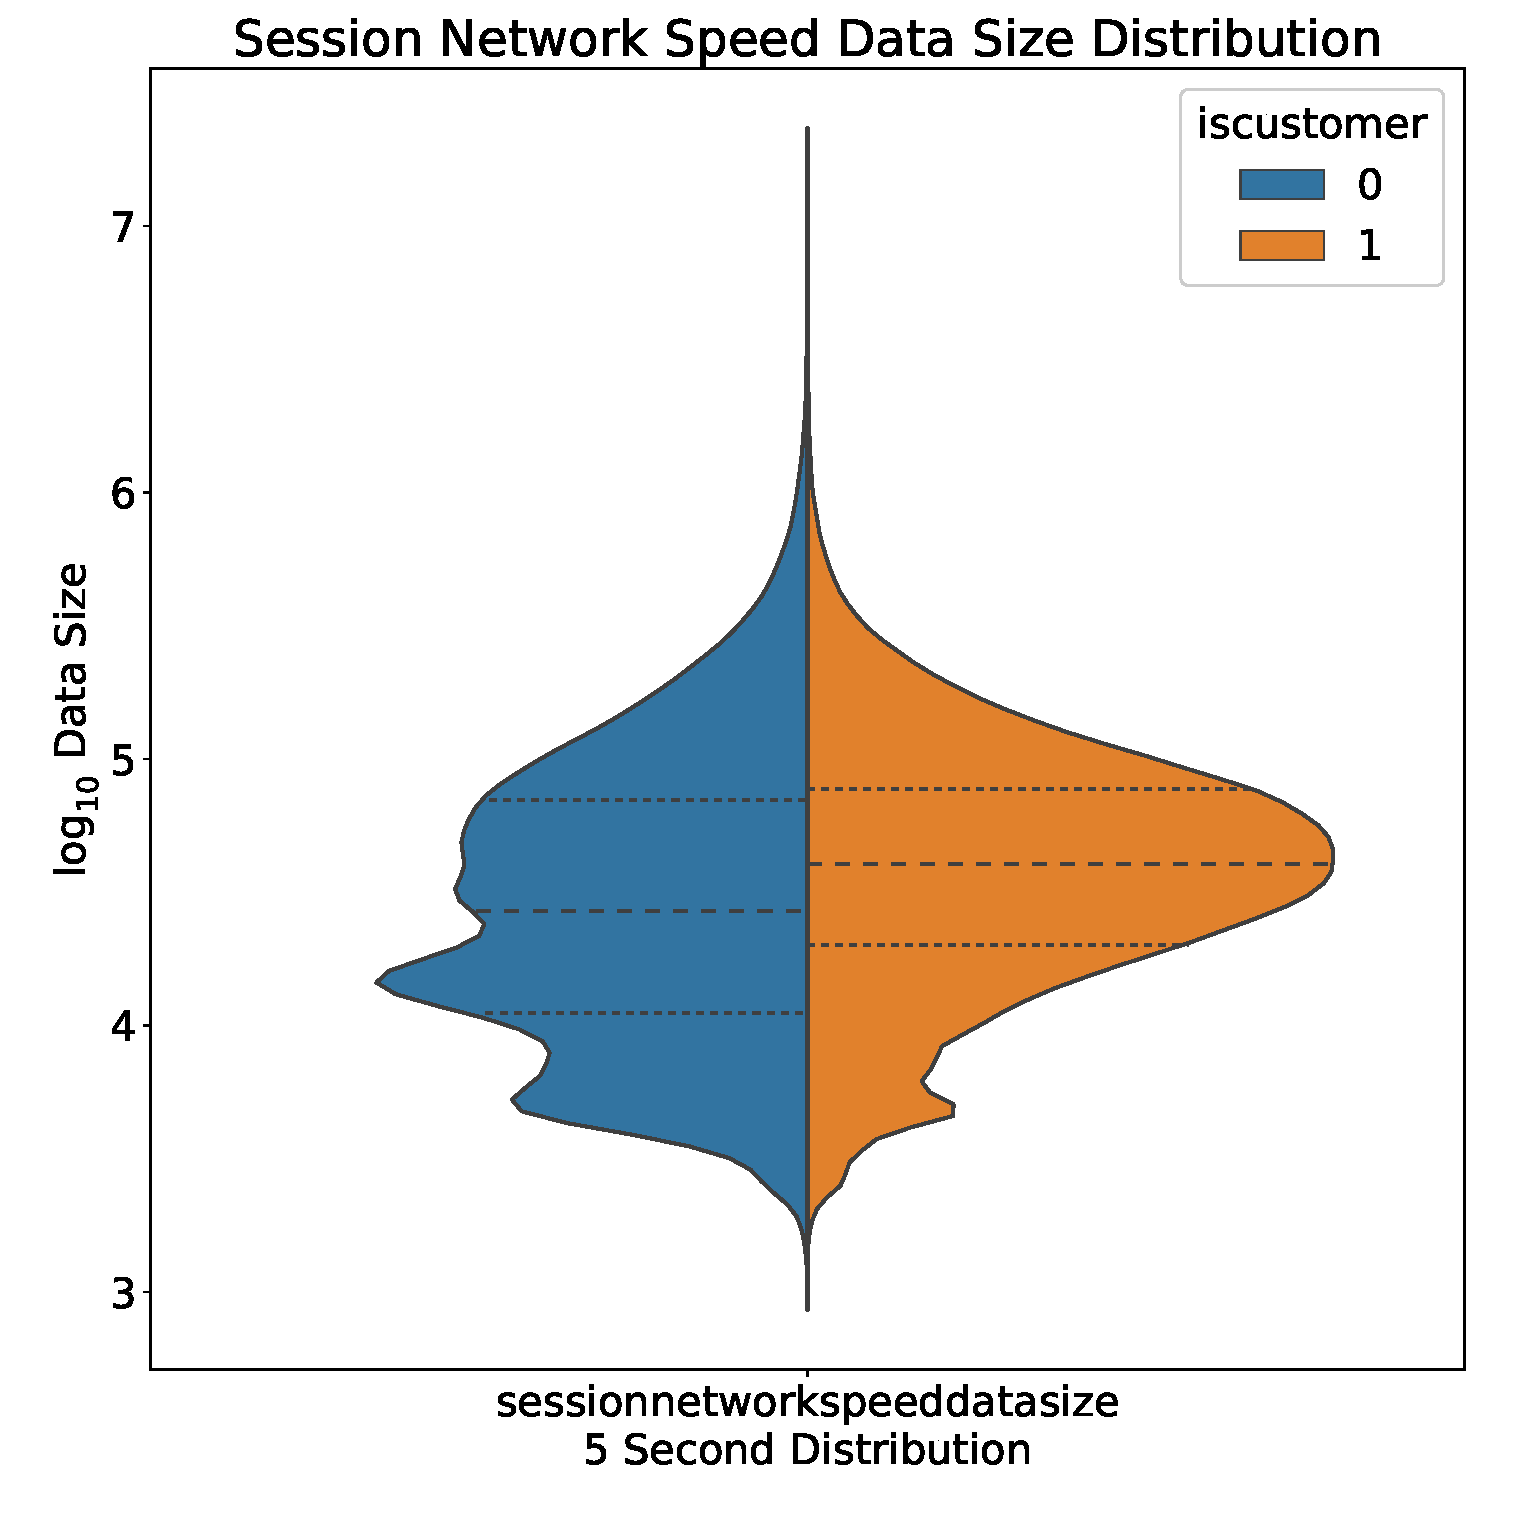
\includegraphics[width=1\textwidth]{fig/violin5.eps}
        \end{figure}
        \end{column}%
        \hfill%
        \begin{column}{.33\textwidth}
        \begin{figure}
            \centering
            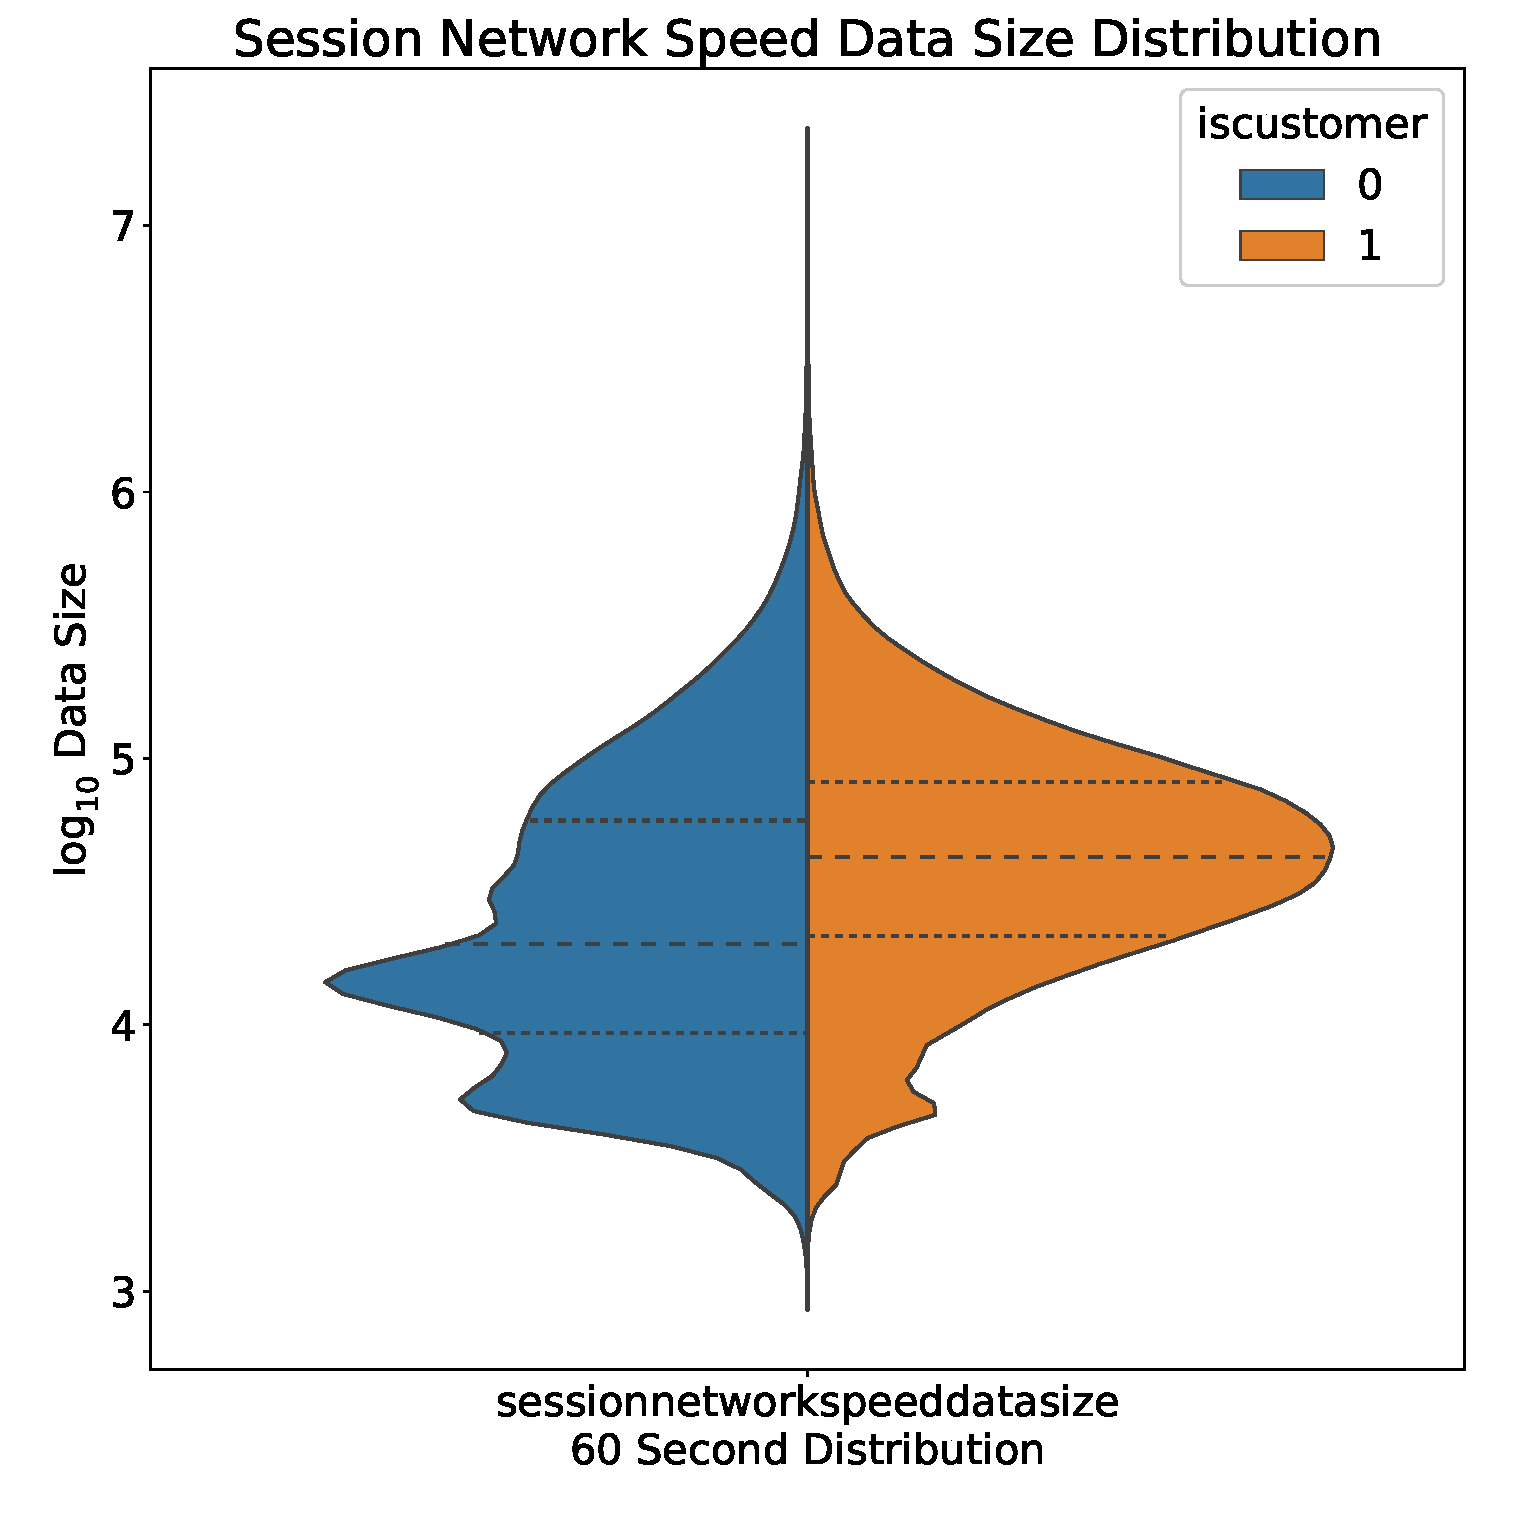
\includegraphics[width=1\textwidth]{fig/violin60.eps}
        \end{figure}        
        \end{column}%
        \begin{column}{.33\textwidth}
        \begin{figure}
            \centering
            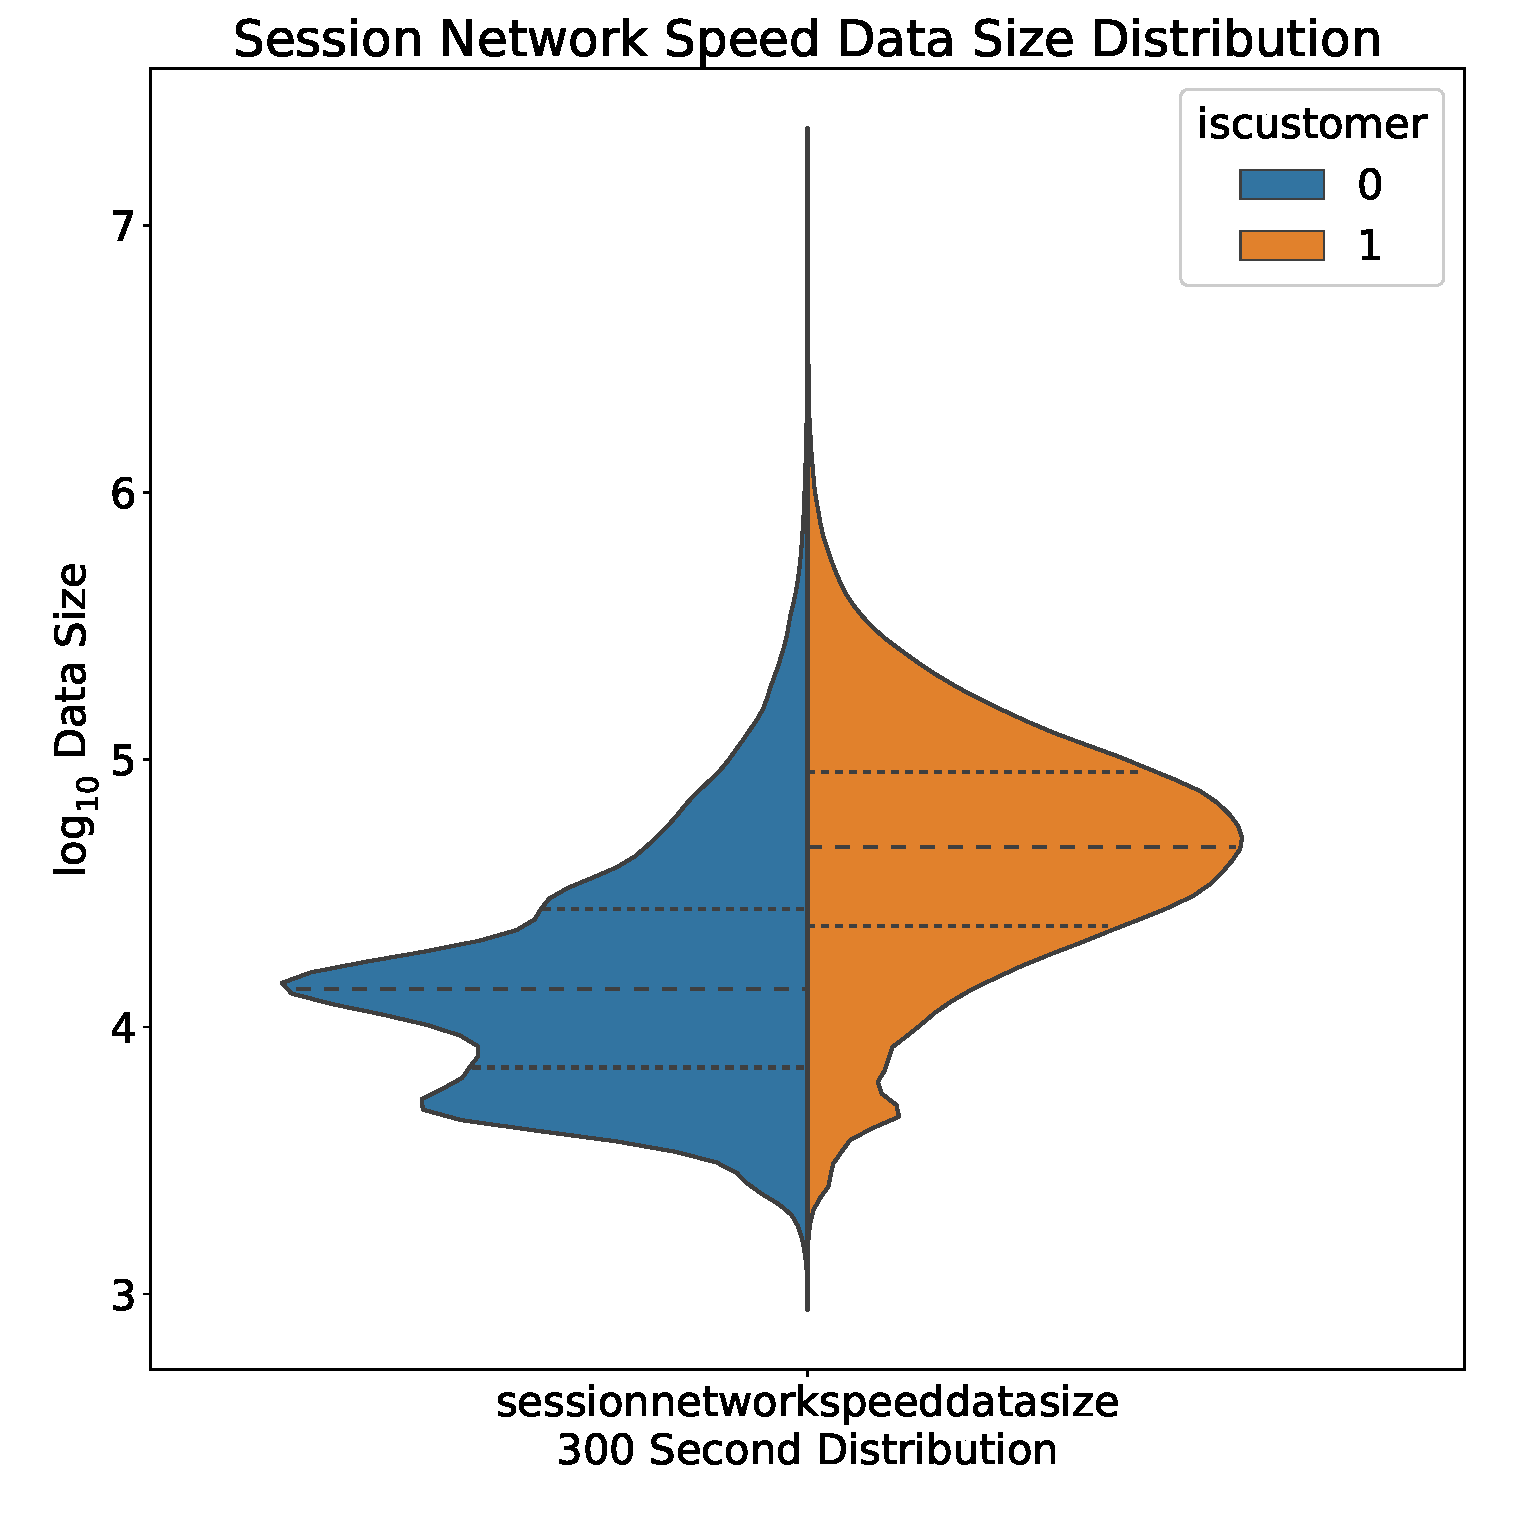
\includegraphics[width=1\textwidth]{fig/violin300.eps}
        \end{figure}        
        \end{column}%        
    \end{columns}
    
}

\frame{
    \frametitle{Data examination II}
        \begin{columns}[T] % align columns
        \begin{column}{.48\textwidth}
        \begin{figure}
            \centering
            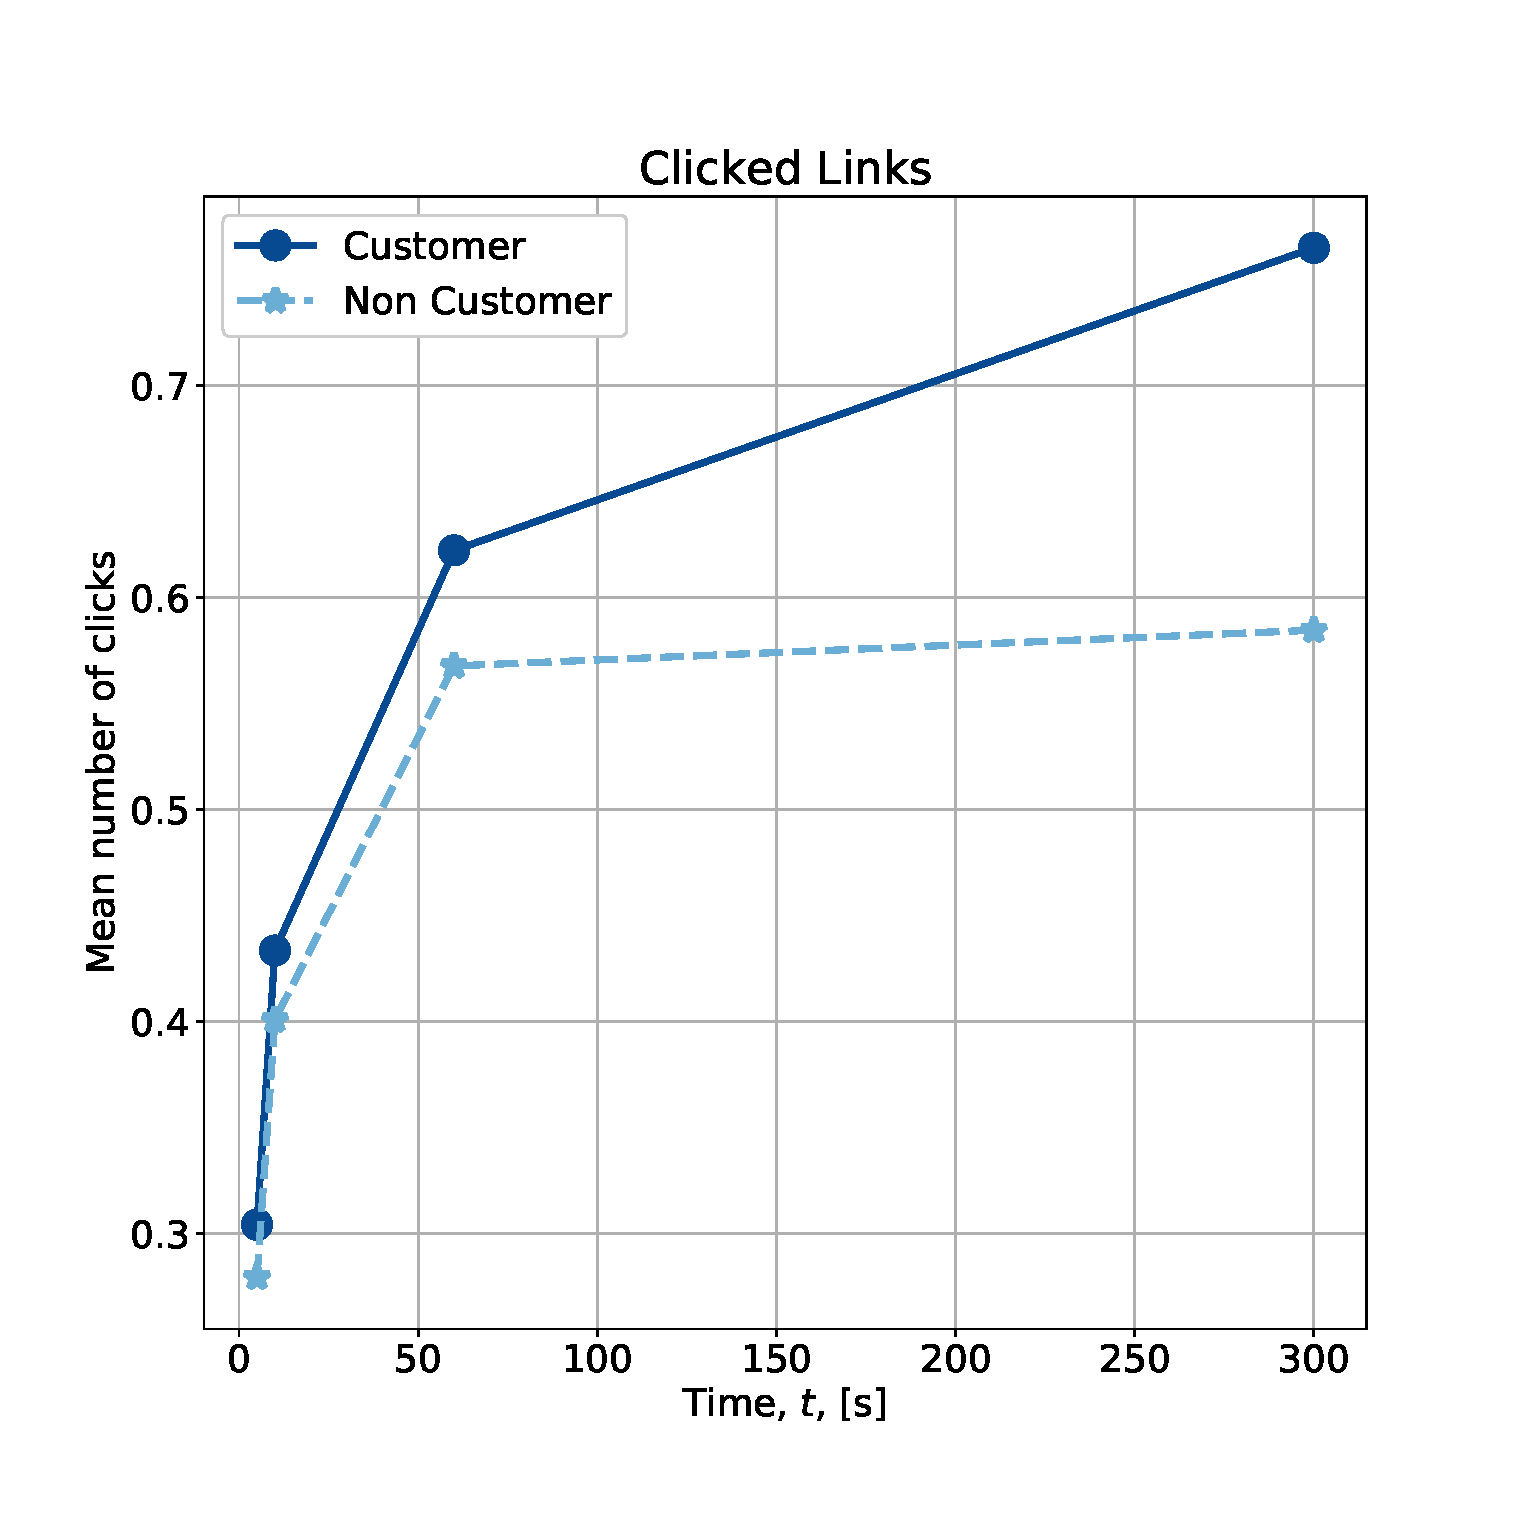
\includegraphics[width=1\textwidth]{fig/clicklinks.eps}
        \end{figure}
        \end{column}%
        \hfill%
        \begin{column}{.48\textwidth}
        \begin{figure}
            \centering
            \includegraphics[width=1\textwidth]{fig/pagenum.eps}
        \end{figure}        
        \end{column}%
    \end{columns}
   
}

\section{Model Justifications}
\frame{
    \frametitle{Interpretability is key}
    We created two models, that is, logistic regression and random forest, both of which are interpretable
    \begin{enumerate}
        \item Logistic Regression was used as a baseline.
        \item It was hypothesised that a Random Forest classifier would be favourable due to the amount of categorical features.
    \end{enumerate}
}

\subsection{Logistic Regression}

\frame{
    \frametitle{Why use Logistics Regression as a baseline?}
    \begin{itemize}
        \item Easy to fit
        \item Intuitive and interpretable
        \item Does not assume anything about the covariances and distributions whereas, conversely, LDA assumes Gaussianity and equal covariance structures.
    \end{itemize}
}

\frame{
    \frametitle{Logistic Regression Recap}
    \begin{itemize}
        \item Idea is to optimise the log-odds function directly
        \begin{itemize}
            \item $\log\,\left[ \dfrac{P\left(\mathit{visitor}=\textcolor{blue}{\mathit{customer}}\right)}{P\left(\mathit{visitor}=\textcolor{red}{\mathit{non\_customer}}\right)}\right] = \beta_0 + \mathbf{x} \beta$
        \end{itemize}
        \item Can be solved by maximum-likelihood
        \item Since the logarithm is concave, in practice, we choose to optimise maximise the log-likelihood which in the case of logistic regression, for a binary classification, becomes
    \end{itemize}
    Let $\boldsymbol{\theta} = \left\{\beta_0, \beta\right\}$
    \begin{equation*}
    \begin{split}
       \boldsymbol{\theta}^{\ast} &= \argmax_{\beta_0, \beta} \log \left(L(\beta_0, \beta) \right) \\
       &= \argmax_{\beta_0, \beta} \sum_{i} \left[ \mathds{1}(\mathbf{x}_i = \textcolor{blue}{\mathit{customer}}) (\beta_0 + \mathbf{x}_i \beta) - \log( 1 + \exp\left( \beta_0 + \mathbf{x}_i \beta \right) \right],
    \end{split}
    \end{equation*}
where $\mathds{1}$ denotes an indicator function and $i$ runs over observations. Optimisation tractable with any method for numerical optimisation. We utilised \texttt{sklearn}'s implementation.
}
\subsection{Random Forest}
\frame{
    \frametitle{Why use a Random Forest Classifier?}
    \begin{enumerate}
        \item Tree-based methods work well with categorical features unless the categorical features have a have cardinality.
        \item Allows for multiple ways of estimating feature importance:
        \begin{itemize}
            \item Based on Gini index: The improvement in the split-criterion at each split is
accumulated over all the trees for each variable.
            \item Based on Out-of-Bag (OOB) samples: Done by permuting the values of the variables one by one after which one can assess the accuracy impact the permutations impose on the model.
        \end{itemize}
        \item Code can be parallelised since the trees are independent. \textbf{WIN}
        \item Multiple efficient off-the-shelf implementations exists within common machine learning libraries for python. We again used \texttt{sklearn}'s.
    \end{enumerate}
}

\frame{
    \frametitle{Recap of Random Forest Algorithm}
    \begin{enumerate}
        \item Define number of trees, $B$. Common is to pick $B$ equal to a few hundred. 
        \item For $b=1$ to $B$ repeat steps (a) - (b)
        \begin{enumerate}
            \item[(a)] Bootstrap $N$ random samples from the data.
            \item[(b)] Repeat until minimum node size $n_{\mathrm{min}}$ reached without pruning:
            \begin{itemize}
                \item Take a random sample without replacement of $m$ variables (where $m$ is less than the total number of features) 
                \item Construct the first Classification Tree partition of the data by picking the optimal split among the $m$ features
            \end{itemize}
        \end{enumerate}
        \item Return $B$ trees
    \end{enumerate}
}

\section{Results}

\subsection{Model Selection}
\frame{
    \frametitle{K-fold Cross-validation}
    \begin{figure}
    \centering
    \threeFoldCV
    \end{figure}
}

\frame{
    \frametitle{Elaboration on model selection}
    \begin{itemize}
        \item We utilised a 2-fold cross-validation in order to tune the models' hyperparameters.
        \item Such a low value of $K$ due to the amount of training data, and partly, because we needed to finish the project under the inevitable time constraints.
        \item One could easily have tried to use information criteria such as Akaike's information Criteria (AIC) or Bayesian information Criteria (BIC) instead of cross-validation for this problem.
    \end{itemize}
}

\subsection{Model Assessment}

\frame{
    \frametitle{Logistic Regression vs. Random Forest}
\onslide<1->{
\resizebox{\textwidth}{!}{
\begin{tabular}{l|cccc|cc|c|c|l|cccc|cc|c}
  \textbf{LR}     & TN & TP & FN & FP & TN\% & TP\% & Acc\%   &\cellcolor{\brilliantBlue}& \textbf{RF}     & TN & TP & FN & FP & TN\% & TP\% & Acc\%   \\ \hline
0s   &  171k  &   173k    &   62k    &  94k  &    64      &     74     & 69  &\cellcolor{\brilliantBlue}&0s   &  177k  &   175k    &   59k    &  89k  &    67      &     75     & 70   \\
5s   &  190k  &  174k  &  60k  &  76k  &     71     &     74     & 73 & \cellcolor{\brilliantBlue}& 5s   &  205k  &  198k  &  35k  &  60k  &     77     &     84     & \textbf{\textcolor{\brilliantBlue}{81}}\\
60s  &  191k  &  213k  &  54k  &  42k  &   82     &    80      & \textbf{\textcolor{\brilliantBlue}{81}} &\cellcolor{\brilliantBlue} & 60s  &  191k  &  232k  &  35k  &  41k  &   82     &    87      & 85 \\ 
300s &  170k  &  263k  &  45k  &   23k   &    88      &    85      & 87 &\cellcolor{\brilliantBlue}&300s &  170k  &  274k  &  34k  &   23k   &    88      &    89      & 89\\ 
\end{tabular}
}
}
\onslide<2->{
    \begin{columns}[T] % align columns
        \begin{column}{.48\textwidth}
        \begin{figure}
            \centering
            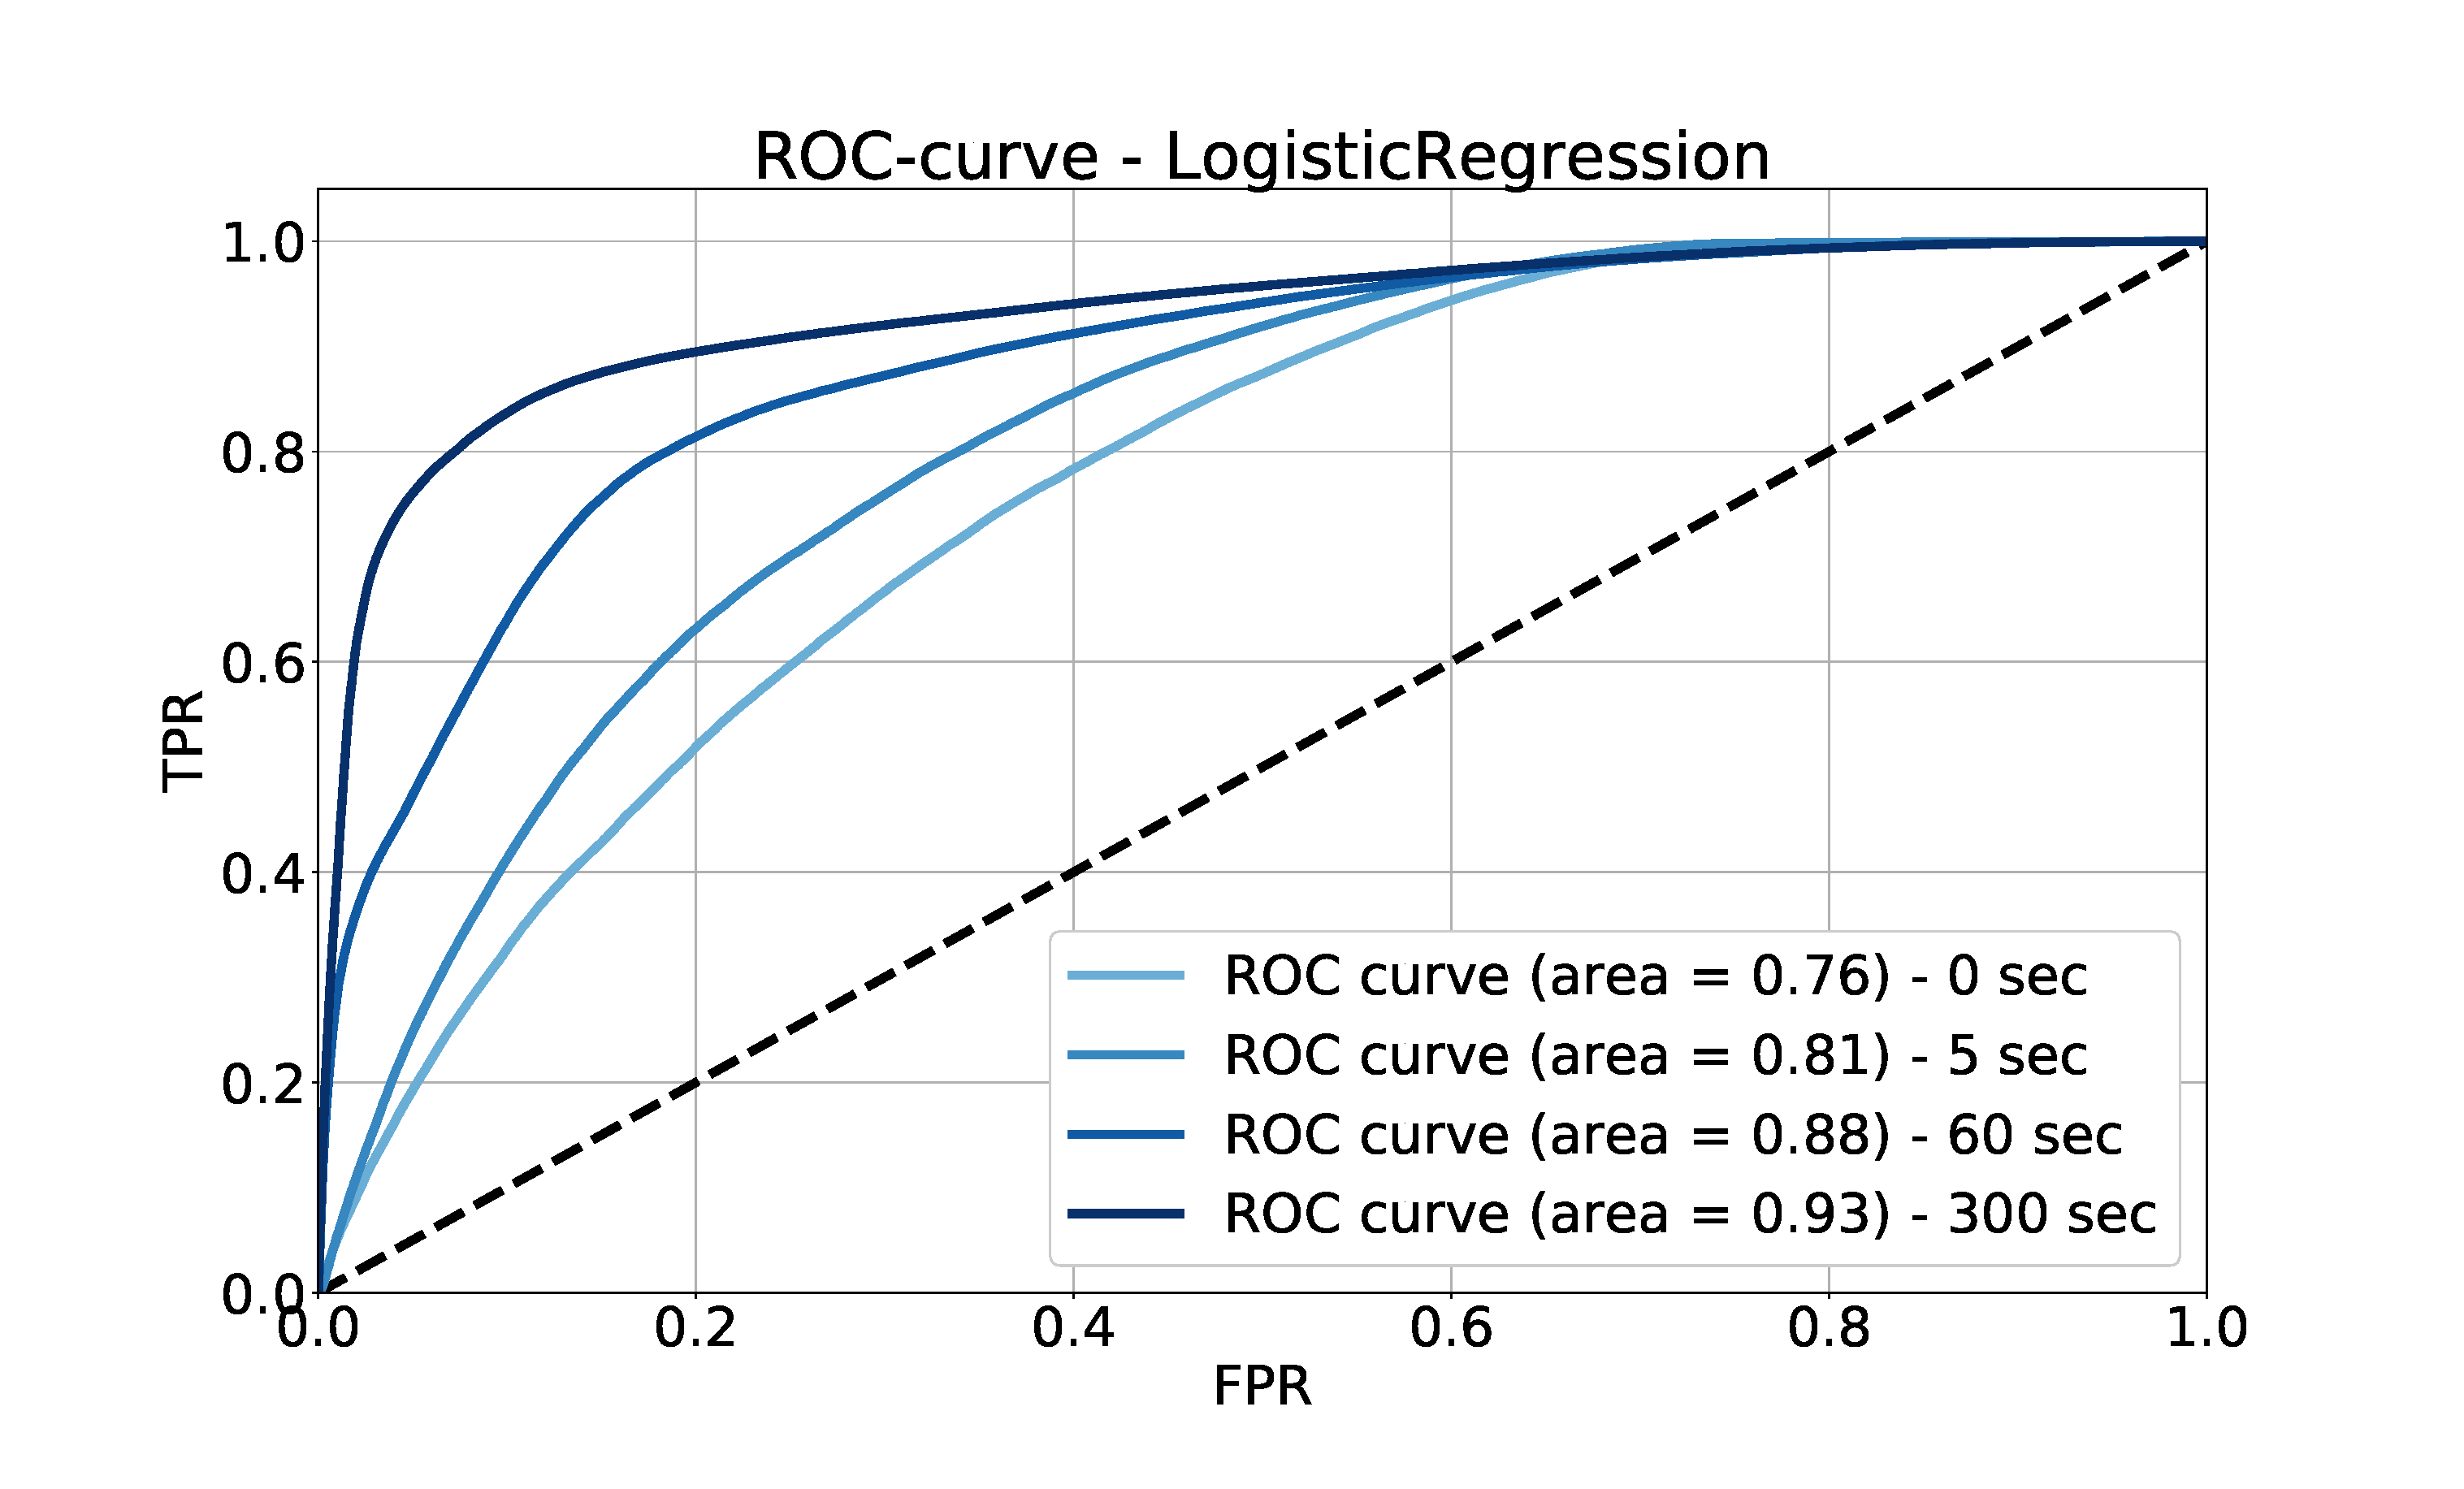
\includegraphics[width=0.95\textwidth]{fig/ROC_LogisticRegression.eps}
        \end{figure}
        \end{column}%
        \hfill%
        \begin{column}{.48\textwidth}
        \begin{figure}
            \centering
            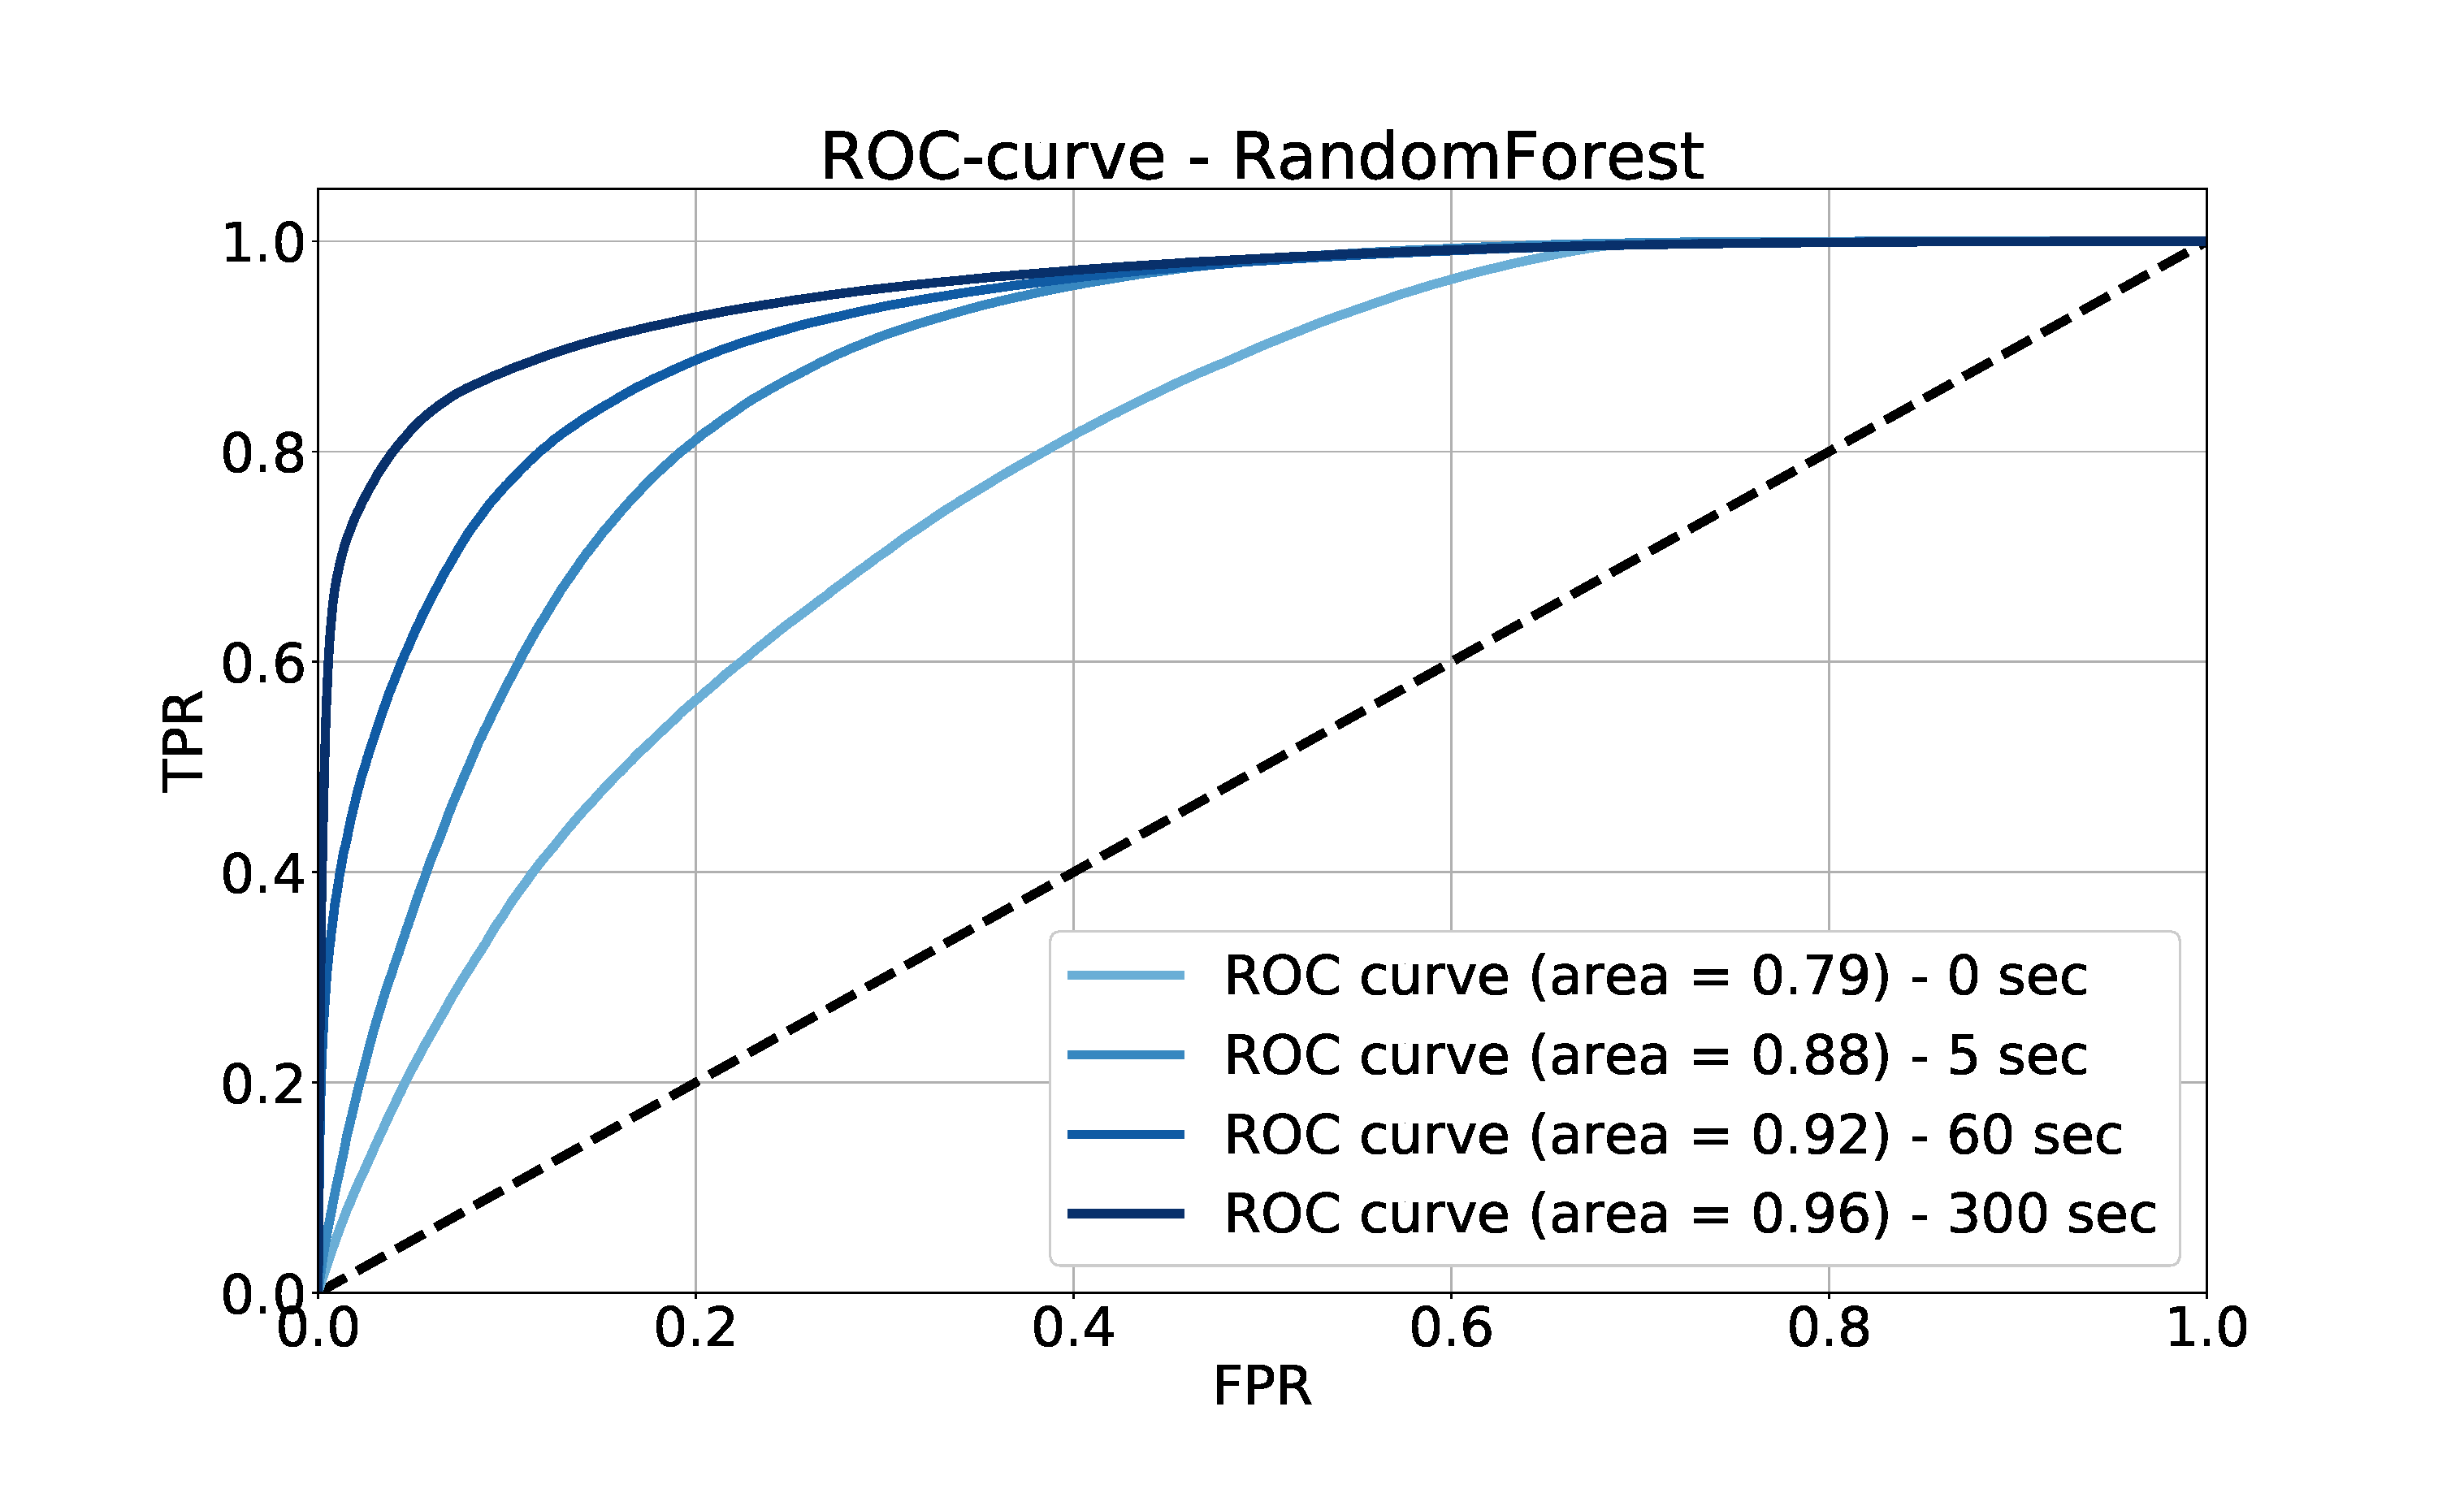
\includegraphics[width=0.95\textwidth]{fig/ROC_RandomForest.eps}
        \end{figure}        
        \end{column}%
    \end{columns}
}
}

\frame{
    \frametitle{Temporal Model Comparison - Random Forest}
    \begin{columns}[T] % align columns
        \begin{column}{.48\textwidth}
        \color{teal}\rule{\linewidth}{4pt}
        0 seconds / initial
        \begin{figure}
            \centering
            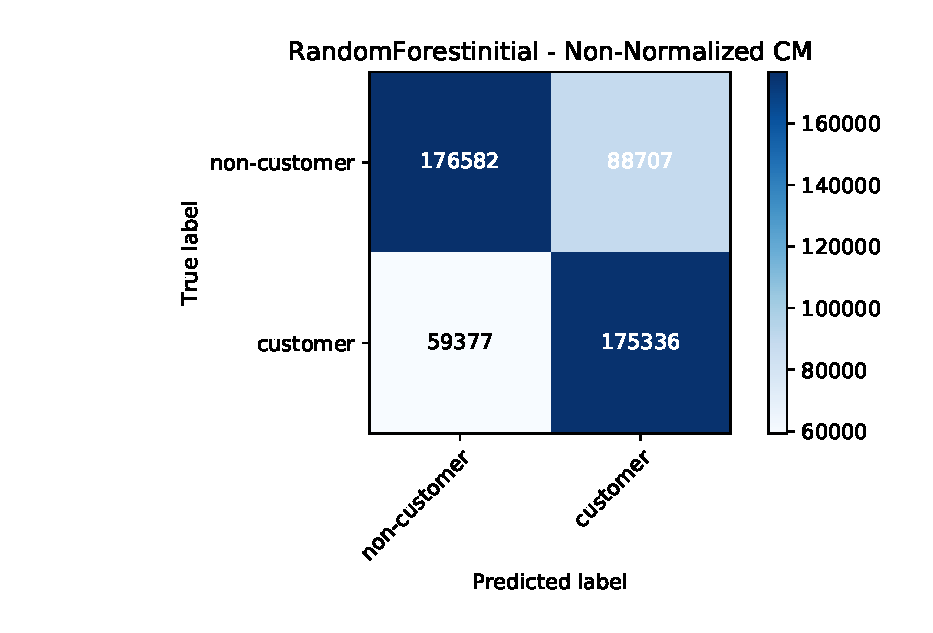
\includegraphics[width=1\textwidth]{fig/RandomForestinitial.eps}
        \end{figure}
        \end{column}%
        \hfill%
        \begin{column}{.48\textwidth}
        \color{blue}\rule{\linewidth}{4pt}
        5 seconds
        \begin{figure}
            \centering
            \includegraphics[width=1\textwidth]{fig/RandomForest5sec.eps}

        \end{figure}        
        \end{column}%
    \end{columns}
    }
    
\section{Discussion}

\subsection{Feature Importance}

\frame{
    \frametitle{Feature Importance}
    \begin{figure}
        \centering
        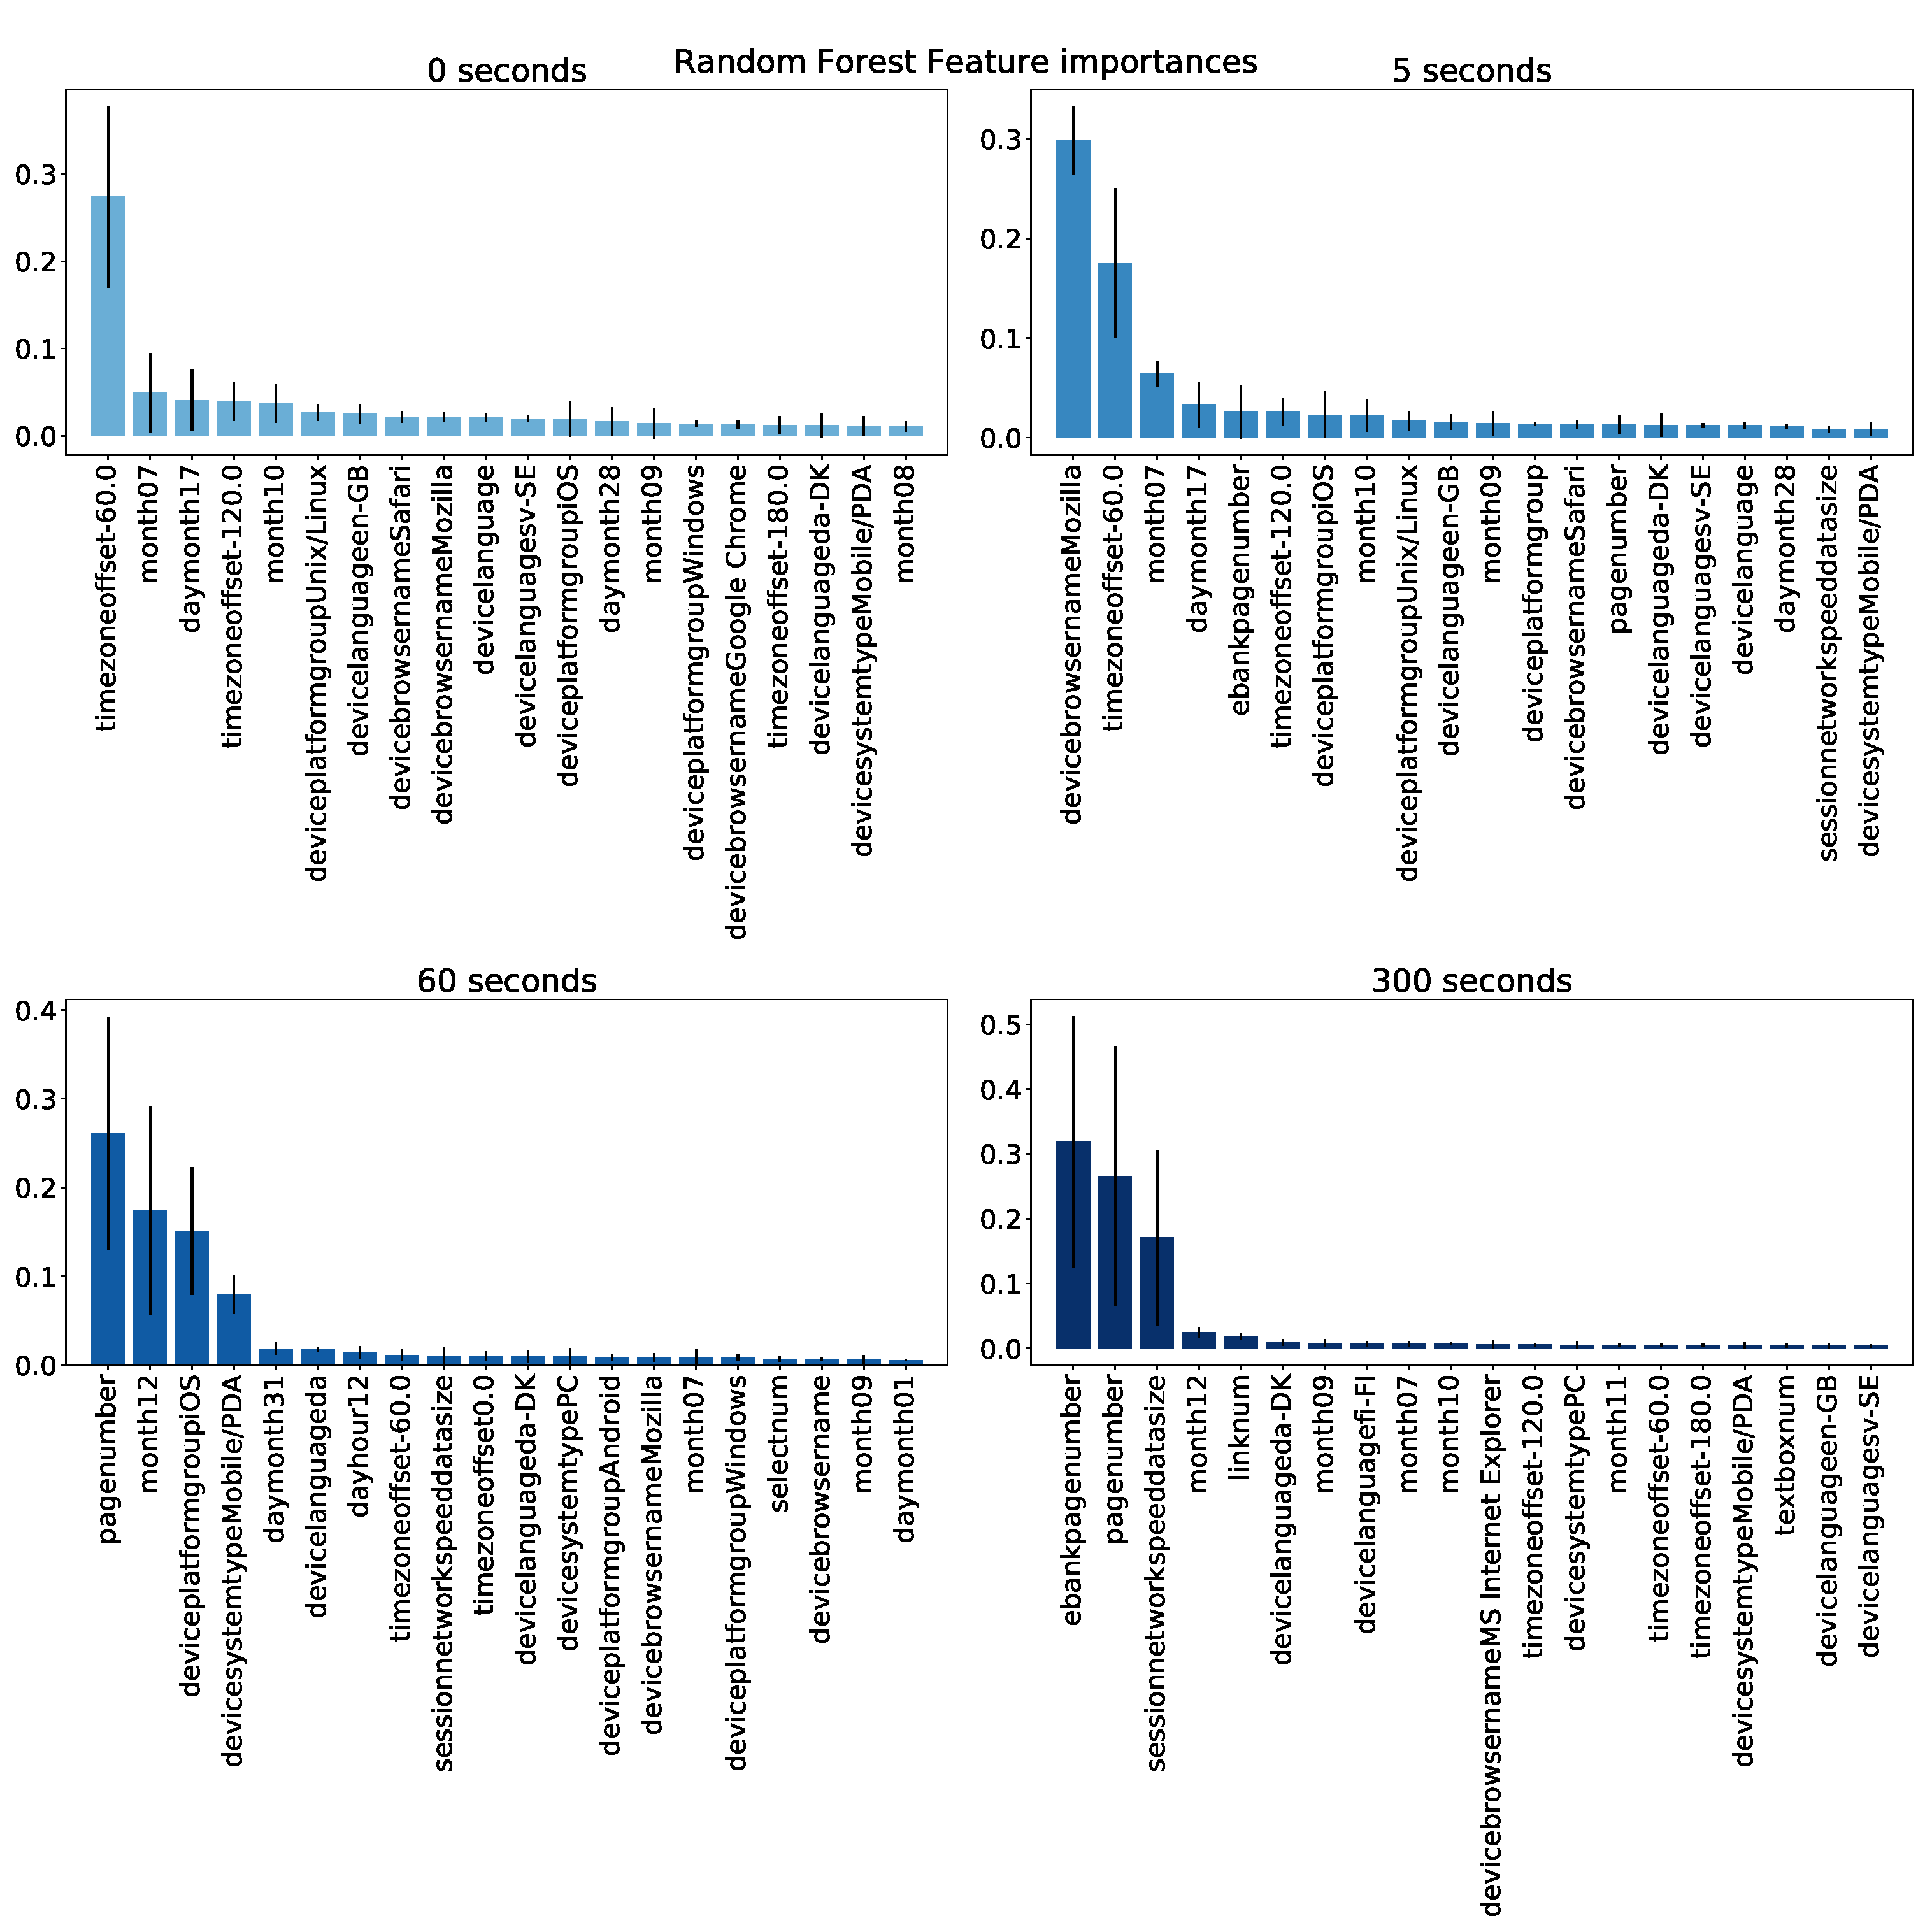
\includegraphics[height=1.03\textheight]{fig/RandomForests_feature_importances.eps}
    \end{figure}
}
\section{Conclusion}

\frame{
    \frametitle{Final remarks and outlook}
    \begin{itemize}
        \item More data $\rightarrow$ better predictions (as anticipated)
        \item Danske Bank efficiently can get an indication as to whether or not a visitor of their web-page is a customer of not. This allows for providing the visitor with tailored links, e.g., by providing customers with quick means of accessing the eBank etc.
        \item Using a Random Forest classifier trained on 500.000 sessions for the 5s dataset, using a 2-Fold CV for model selection, we were able to achieve a test accuracy of \textbf{\textcolor{blue}{81\%}}
        \item It would be beneficial to create ML models based on user-stories defined in collaboration with the users (internal \& external). For instance through design thinking.
        \begin{itemize}
            \item Opening up for the possibility of using \textsc{Celebrus} in conjunction with public data, and other Danske Bank data assets, to meet user demands through prolific data modelling.
            \item Note that users here may have totally different needs:
            \begin{enumerate}
                \item could be an internal employee trying to do customer segmentation
                \item could be an external web-page visitor who finds the UX part of \url{https://danskebank.dk} confusing.
            \end{enumerate}
        \end{itemize}
    \end{itemize}
     
}

%================================================
%===  Define the contact details
\newcommand\contactTable{ %
  \begin{tabular}{lr}
    \multicolumn{2}{l}{Victor Elkjær Birk \& William Frisch Møller} \\ 
    \multicolumn{2}{l}{\textbf{Technical University of Denmark (DTU)}} \\ \midrule
    \textbf{Email}    & victor [dot] elkjaer [at] gmail [dot] com \\
     & william [dot] frisch [dot] moller [at] gmail [dot] com \\
    \textbf{LinkedIn} & \href{https://www.linkedin.com/in/vebirk/}{vebirk} \\
    & \href{https://www.linkedin.com/in/wfm1996}{wfm1996} \\
    \textbf{Website} &  \url{https://www.victorelkjaer.com}  \\
  \end{tabular}
}%


\frame[dtuwhitelogo, bgfilename=dtu_bg_nano]{
  \begin{tikzpicture}[remember picture,overlay]
    \node[fill=black, fill opacity=0.9, 
          text=white, text opacity=1.0,
          rounded corners=5pt, 
          font=\scriptsize] at (current page.center) {\contactTable};
  \end{tikzpicture}
}


\end{document}